%\documentclass[12pt]{report}
%
%\usepackage{amsfonts}
%\usepackage{amsmath}
%\usepackage{geometry}
%\usepackage{listings}
%\usepackage[dvipsnames]{xcolor}
%\usepackage{graphicx}
%%\usepackage{wrapfig}
%\usepackage{subcaption}
%%\usepackage{hyperref}
%\usepackage{setspace}
%
%\definecolor{codegreen}{rgb}{0,0.6,0}
%\definecolor{codegray}{rgb}{0.5,0.5,0.5}
%\definecolor{codepurple}{rgb}{0.58,0,0.82}
%\definecolor{backcolour}{rgb}{0.95,0.95,0.92}
% 
%\lstdefinestyle{mystyle}{
%    emph={self, Equation, loop, BlackHole2D,__init__, initialize, BlackHole, Application, Group},
%    emphstyle=\color{PineGreen},
%    commentstyle=\color{blue},
%    keywordstyle={\color{BrickRed}\bfseries},
%    numberstyle=\color{codegray},
%    stringstyle=\color{codepurple},
%    breakatwhitespace=false,         
%    breaklines=true,                 
%    captionpos=b,                    
%    keepspaces=true,                 
%    numbers=left,                    
%    numbersep=5pt,                  
%    showspaces=false,                
%    showstringspaces=false,
%    showtabs=false,                  
%    tabsize=2
%}
%
%\newgeometry{margin=1in}
%\setlength\parindent{0pt}
%
%\DeclareMathOperator{\grad}{\overset{\rightharpoonup}\nabla}
%
%\begin{document}
%
%\doublespacing
%\linespread{2}
%\lstset{style=mystyle}

\chapter{Simulation Solution}
\label{chap:sim}

\section{Smoothed Particle Hydrodynamics}

Since we model neutron stars as a fluid, in order to simulate the collision of a primordial black hole with a neutron star, we need to use computational fluid dynamics, more specifically, smoothed particle hydrodynamics (SPH). Smoothed particle hydrodynamics was initially developed in 1977 for simulating spherically asymmetric stars \cite{origsph}. A major assumption in the modelling of stars is that they are spherically symmetric, however, there are a lot of cases where this is not true. For example the collapse of a protostar will be very inhomogeneous, or if the star has a large angular momentum or strong magnetic fields, the star will be considerably deformed \cite{origsph}. \\

Smoothed particle hydrodynamics has since been extended more generally so it can be applied outside of astrophysics to areas such as solid mechanics and fluid dynamics. In essence, smoothed particle hydrodynamics uses similar methods of N-body code -- the continuous media is represented as a set of particles, and the equations are solved numerically. Mathematically, the particles represent the points at which the properties of the fluid are calculated, and the rest can then be interpolated. Physically, the particles are simply a subset of all the particles in the system \cite{newsph}. One of the biggest advantages of smoothed particle hydrodynamics is that it is mesh-free, unlike most computational fluid dynamics methods. Therefore, it is very useful for interactions between different types of particles, and for free surface simulations. \\

Typically, smoothed particle hydrodynamics uses a nearest neighbour scheme for calculating the changes in a particle's properties. This is done by using a cubic Hermite spline to interpolate properties within a radius of twice the smoothing length of a particular particle. A cubic Hermite spline is a set of cubic polynomials specified by its values, and the values of its first derivative at the boundaries of the interval.

\subsection{PySPH}
The simulations were conducted with PySPH \cite{pysph}, open source SPH code written in Python and compiled in Cython. This allows a majority of the code to be written in pure Python, but is then converted to high performance Cython code to run at speeds closer to C and FORTRAN. For further optimizations, PySPH can run in parallel with OpenMP and MPI to take advantage of multiple cores / threads. One of the main reasons for choosing PySPH is that it allows the flexibility of user defined classes and equations which was needed to incorporate the primordial black hole.

\section{Code}

In order to simulate a primordial black hole collision with a neutron star we must first write a class to include the acceleration. The acceleration of course is just
\begin{align*}
\overset{\rightharpoonup}a &= - \frac{1}{m_{part}} \grad \Phi.
\end{align*}

Within the coordinates in PySPH
\begin{align*}
\overset{\rightharpoonup}a &= \frac{-m}{\left( x^2 + s^2 + (y + v\tau)^2 \right)^{3/2}} \left( \begin{matrix}
x \\
y+v \tau
\end{matrix}
\right)
\end{align*}
with $G = 1$, $\tau = t-t\_hit$, and $s$ a softening length so the solution does not diverge at $\tau = 0$ at the origin. The mass of the particle is also omitted in the simulation because PySPH uses acceleration per unit mass. In the class function (Figure \ref{fig:blackholeclass}) the velocity is hard coded to be $1$, and the parameter \emph{t\_hit} is used to offset the collision of the primordial black hole since the simulation starts at $t = 0$. \\

Now that the class function has been written, it can be called within the equations block of the main file, \emph{blackhole.py}. Figure \ref{fig:blackhole} shows the important sections of \emph{blackhole.py}; first the acceleration equation is imported, and the values for the simulation are specified in the preamble. Then, the black hole can be added to the equations group in the main acceleration block. The included example \emph{hydrostatic\_tank.py} was used as the base for \emph{blackhole.py}, it was the most useful starting point -- it is a 2D tank filled with fluid, and includes the force of gravity. \\

\begin{figure}[p]
\lstinputlisting[language=Python, lastline=18]{../BlackHoleEquation.py}
\caption[Acceleration addition due to a primordial black hole]{Class file for adding the acceleration due to the primordial black hole, \emph{BlackHoleEquation.py}.}
\label{fig:blackholeclass}
\end{figure}

\begin{figure}[p]
  \lstinputlisting[language=Python, firstnumber=19, firstline=19, lastline=21]{../blackhole.py}
  \lstinputlisting[language=Python, firstnumber=40, firstline=40, lastline=59]{../blackhole.py}
  \lstinputlisting[language=Python, firstnumber=82, firstline=82, lastline=82]{../blackhole.py}
  \lstinputlisting[language=Python, firstnumber=171, firstline=171, lastline=173]{../blackhole.py}
  \lstinputlisting[language=Python, firstnumber=194, firstline=194, lastline=195]{../blackhole.py}
  \lstinputlisting[language=Python, firstnumber=212, firstline=212, lastline=217]{../blackhole.py}
 \caption{Modifications of the hydrostatic tank example, \emph{blackhole.py}.}
 \label{fig:blackhole}
\end{figure}

The parameters of the simulation were mostly the same as what were used to generate the images of the analytic solution -- everything set equal to unity -- with the exceptions of \emph{t\_hit} $= 200$, and $s=0.01$. The reason \emph{t\_hit} is so large is due to how the particles are initially placed. They are simply placed on a grid with spacing $dx$; once the simulation starts, gravity pulls the surface down attempting to equilibrate to a linear pressure gradient. However, since the fluid is not at equilibrium, the surface undergoes harmonic motion and is slowly dampened to equilibrium and so the long \emph{t\_hit} is an attempt to dampen out a majority of the oscillations. \\

Determining the dimensions of the tank required a considerable amount of care. If the tank was too narrow, the walls at the edges would reflect the initial waves which would then start to interfere with the secondary waves. This caused erroneous results in the energy calculations during testing. Similarly, if the tank was too shallow, the waves resembled shallow water waves instead of deep, as in our model. And of course, if the tank was needlessly large, it greatly affected the computation time of the simulation. In the end, $Lx = 120$, $Ly = 15$, and $dx = 0.075$ were decided on.

\section{Simulation Results}

In total the simulation took about 330 CPU hours over the course of three days. The resulting surface waves from the collision can be seen in Figure \ref{fig:simresults}.
\begin{figure}[p]
\centering
\begin{subfigure}{\textwidth}
% GNUPLOT: LaTeX picture with Postscript
\begingroup
  \makeatletter
  \providecommand\color[2][]{%
    \GenericError{(gnuplot) \space\space\space\@spaces}{%
      Package color not loaded in conjunction with
      terminal option `colourtext'%
    }{See the gnuplot documentation for explanation.%
    }{Either use 'blacktext' in gnuplot or load the package
      color.sty in LaTeX.}%
    \renewcommand\color[2][]{}%
  }%
  \providecommand\includegraphics[2][]{%
    \GenericError{(gnuplot) \space\space\space\@spaces}{%
      Package graphicx or graphics not loaded%
    }{See the gnuplot documentation for explanation.%
    }{The gnuplot epslatex terminal needs graphicx.sty or graphics.sty.}%
    \renewcommand\includegraphics[2][]{}%
  }%
  \providecommand\rotatebox[2]{#2}%
  \@ifundefined{ifGPcolor}{%
    \newif\ifGPcolor
    \GPcolorfalse
  }{}%
  \@ifundefined{ifGPblacktext}{%
    \newif\ifGPblacktext
    \GPblacktexttrue
  }{}%
  % define a \g@addto@macro without @ in the name:
  \let\gplgaddtomacro\g@addto@macro
  % define empty templates for all commands taking text:
  \gdef\gplbacktext{}%
  \gdef\gplfronttext{}%
  \makeatother
  \ifGPblacktext
    % no textcolor at all
    \def\colorrgb#1{}%
    \def\colorgray#1{}%
  \else
    % gray or color?
    \ifGPcolor
      \def\colorrgb#1{\color[rgb]{#1}}%
      \def\colorgray#1{\color[gray]{#1}}%
      \expandafter\def\csname LTw\endcsname{\color{white}}%
      \expandafter\def\csname LTb\endcsname{\color{black}}%
      \expandafter\def\csname LTa\endcsname{\color{black}}%
      \expandafter\def\csname LT0\endcsname{\color[rgb]{1,0,0}}%
      \expandafter\def\csname LT1\endcsname{\color[rgb]{0,1,0}}%
      \expandafter\def\csname LT2\endcsname{\color[rgb]{0,0,1}}%
      \expandafter\def\csname LT3\endcsname{\color[rgb]{1,0,1}}%
      \expandafter\def\csname LT4\endcsname{\color[rgb]{0,1,1}}%
      \expandafter\def\csname LT5\endcsname{\color[rgb]{1,1,0}}%
      \expandafter\def\csname LT6\endcsname{\color[rgb]{0,0,0}}%
      \expandafter\def\csname LT7\endcsname{\color[rgb]{1,0.3,0}}%
      \expandafter\def\csname LT8\endcsname{\color[rgb]{0.5,0.5,0.5}}%
    \else
      % gray
      \def\colorrgb#1{\color{black}}%
      \def\colorgray#1{\color[gray]{#1}}%
      \expandafter\def\csname LTw\endcsname{\color{white}}%
      \expandafter\def\csname LTb\endcsname{\color{black}}%
      \expandafter\def\csname LTa\endcsname{\color{black}}%
      \expandafter\def\csname LT0\endcsname{\color{black}}%
      \expandafter\def\csname LT1\endcsname{\color{black}}%
      \expandafter\def\csname LT2\endcsname{\color{black}}%
      \expandafter\def\csname LT3\endcsname{\color{black}}%
      \expandafter\def\csname LT4\endcsname{\color{black}}%
      \expandafter\def\csname LT5\endcsname{\color{black}}%
      \expandafter\def\csname LT6\endcsname{\color{black}}%
      \expandafter\def\csname LT7\endcsname{\color{black}}%
      \expandafter\def\csname LT8\endcsname{\color{black}}%
    \fi
  \fi
    \setlength{\unitlength}{0.0500bp}%
    \ifx\gptboxheight\undefined%
      \newlength{\gptboxheight}%
      \newlength{\gptboxwidth}%
      \newsavebox{\gptboxtext}%
    \fi%
    \setlength{\fboxrule}{0.5pt}%
    \setlength{\fboxsep}{1pt}%
\begin{picture}(8640.00,3600.00)%
    \gplgaddtomacro\gplbacktext{%
      \csname LTb\endcsname%
      \put(682,967){\makebox(0,0)[r]{\strut{}$-4$}}%
      \put(682,1493){\makebox(0,0)[r]{\strut{}$-2$}}%
      \put(682,2020){\makebox(0,0)[r]{\strut{}$0$}}%
      \put(682,2546){\makebox(0,0)[r]{\strut{}$2$}}%
      \put(682,3072){\makebox(0,0)[r]{\strut{}$4$}}%
      \put(814,484){\makebox(0,0){\strut{}$-10$}}%
      \put(2383,484){\makebox(0,0){\strut{}$-5$}}%
      \put(3952,484){\makebox(0,0){\strut{}$0$}}%
      \put(5521,484){\makebox(0,0){\strut{}$5$}}%
      \put(7090,484){\makebox(0,0){\strut{}$10$}}%
    }%
    \gplgaddtomacro\gplfronttext{%
      \csname LTb\endcsname%
      \put(176,2019){\makebox(0,0){\strut{}$y$}}%
      \put(3952,154){\makebox(0,0){\strut{}$x$}}%
      \csname LTb\endcsname%
      \put(7692,704){\makebox(0,0)[l]{\strut{}$0.99$}}%
      \put(7692,1142){\makebox(0,0)[l]{\strut{}$1$}}%
      \put(7692,1581){\makebox(0,0)[l]{\strut{}$1.01$}}%
      \put(7692,2019){\makebox(0,0)[l]{\strut{}$1.02$}}%
      \put(7692,2458){\makebox(0,0)[l]{\strut{}$1.03$}}%
      \put(7692,2896){\makebox(0,0)[l]{\strut{}$1.04$}}%
      \put(7692,3335){\makebox(0,0)[l]{\strut{}$1.05$}}%
      \put(8286,2019){\makebox(0,0){\strut{} $\rho$}}%
    }%
    \gplbacktext
    \put(0,0){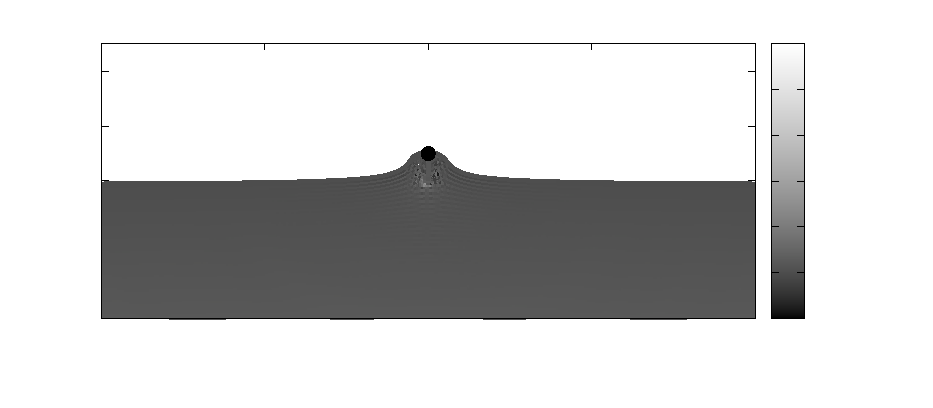
\includegraphics{./Sim199}}%
    \gplfronttext
  \end{picture}%
\endgroup

\caption{$\tau = -1$}
\end{subfigure} \\
\begin{subfigure}{\textwidth}
% GNUPLOT: LaTeX picture with Postscript
\begingroup
  \makeatletter
  \providecommand\color[2][]{%
    \GenericError{(gnuplot) \space\space\space\@spaces}{%
      Package color not loaded in conjunction with
      terminal option `colourtext'%
    }{See the gnuplot documentation for explanation.%
    }{Either use 'blacktext' in gnuplot or load the package
      color.sty in LaTeX.}%
    \renewcommand\color[2][]{}%
  }%
  \providecommand\includegraphics[2][]{%
    \GenericError{(gnuplot) \space\space\space\@spaces}{%
      Package graphicx or graphics not loaded%
    }{See the gnuplot documentation for explanation.%
    }{The gnuplot epslatex terminal needs graphicx.sty or graphics.sty.}%
    \renewcommand\includegraphics[2][]{}%
  }%
  \providecommand\rotatebox[2]{#2}%
  \@ifundefined{ifGPcolor}{%
    \newif\ifGPcolor
    \GPcolorfalse
  }{}%
  \@ifundefined{ifGPblacktext}{%
    \newif\ifGPblacktext
    \GPblacktexttrue
  }{}%
  % define a \g@addto@macro without @ in the name:
  \let\gplgaddtomacro\g@addto@macro
  % define empty templates for all commands taking text:
  \gdef\gplbacktext{}%
  \gdef\gplfronttext{}%
  \makeatother
  \ifGPblacktext
    % no textcolor at all
    \def\colorrgb#1{}%
    \def\colorgray#1{}%
  \else
    % gray or color?
    \ifGPcolor
      \def\colorrgb#1{\color[rgb]{#1}}%
      \def\colorgray#1{\color[gray]{#1}}%
      \expandafter\def\csname LTw\endcsname{\color{white}}%
      \expandafter\def\csname LTb\endcsname{\color{black}}%
      \expandafter\def\csname LTa\endcsname{\color{black}}%
      \expandafter\def\csname LT0\endcsname{\color[rgb]{1,0,0}}%
      \expandafter\def\csname LT1\endcsname{\color[rgb]{0,1,0}}%
      \expandafter\def\csname LT2\endcsname{\color[rgb]{0,0,1}}%
      \expandafter\def\csname LT3\endcsname{\color[rgb]{1,0,1}}%
      \expandafter\def\csname LT4\endcsname{\color[rgb]{0,1,1}}%
      \expandafter\def\csname LT5\endcsname{\color[rgb]{1,1,0}}%
      \expandafter\def\csname LT6\endcsname{\color[rgb]{0,0,0}}%
      \expandafter\def\csname LT7\endcsname{\color[rgb]{1,0.3,0}}%
      \expandafter\def\csname LT8\endcsname{\color[rgb]{0.5,0.5,0.5}}%
    \else
      % gray
      \def\colorrgb#1{\color{black}}%
      \def\colorgray#1{\color[gray]{#1}}%
      \expandafter\def\csname LTw\endcsname{\color{white}}%
      \expandafter\def\csname LTb\endcsname{\color{black}}%
      \expandafter\def\csname LTa\endcsname{\color{black}}%
      \expandafter\def\csname LT0\endcsname{\color{black}}%
      \expandafter\def\csname LT1\endcsname{\color{black}}%
      \expandafter\def\csname LT2\endcsname{\color{black}}%
      \expandafter\def\csname LT3\endcsname{\color{black}}%
      \expandafter\def\csname LT4\endcsname{\color{black}}%
      \expandafter\def\csname LT5\endcsname{\color{black}}%
      \expandafter\def\csname LT6\endcsname{\color{black}}%
      \expandafter\def\csname LT7\endcsname{\color{black}}%
      \expandafter\def\csname LT8\endcsname{\color{black}}%
    \fi
  \fi
    \setlength{\unitlength}{0.0500bp}%
    \ifx\gptboxheight\undefined%
      \newlength{\gptboxheight}%
      \newlength{\gptboxwidth}%
      \newsavebox{\gptboxtext}%
    \fi%
    \setlength{\fboxrule}{0.5pt}%
    \setlength{\fboxsep}{1pt}%
\begin{picture}(8640.00,3600.00)%
    \gplgaddtomacro\gplbacktext{%
      \csname LTb\endcsname%
      \put(682,967){\makebox(0,0)[r]{\strut{}$-4$}}%
      \put(682,1493){\makebox(0,0)[r]{\strut{}$-2$}}%
      \put(682,2020){\makebox(0,0)[r]{\strut{}$0$}}%
      \put(682,2546){\makebox(0,0)[r]{\strut{}$2$}}%
      \put(682,3072){\makebox(0,0)[r]{\strut{}$4$}}%
      \put(814,484){\makebox(0,0){\strut{}$-10$}}%
      \put(2383,484){\makebox(0,0){\strut{}$-5$}}%
      \put(3952,484){\makebox(0,0){\strut{}$0$}}%
      \put(5521,484){\makebox(0,0){\strut{}$5$}}%
      \put(7090,484){\makebox(0,0){\strut{}$10$}}%
    }%
    \gplgaddtomacro\gplfronttext{%
      \csname LTb\endcsname%
      \put(176,2019){\makebox(0,0){\strut{}$y$}}%
      \put(3952,154){\makebox(0,0){\strut{}$x$}}%
      \csname LTb\endcsname%
      \put(7692,704){\makebox(0,0)[l]{\strut{}$0.99$}}%
      \put(7692,1142){\makebox(0,0)[l]{\strut{}$1$}}%
      \put(7692,1581){\makebox(0,0)[l]{\strut{}$1.01$}}%
      \put(7692,2019){\makebox(0,0)[l]{\strut{}$1.02$}}%
      \put(7692,2458){\makebox(0,0)[l]{\strut{}$1.03$}}%
      \put(7692,2896){\makebox(0,0)[l]{\strut{}$1.04$}}%
      \put(7692,3335){\makebox(0,0)[l]{\strut{}$1.05$}}%
      \put(8286,2019){\makebox(0,0){\strut{} $\rho$}}%
    }%
    \gplbacktext
    \put(0,0){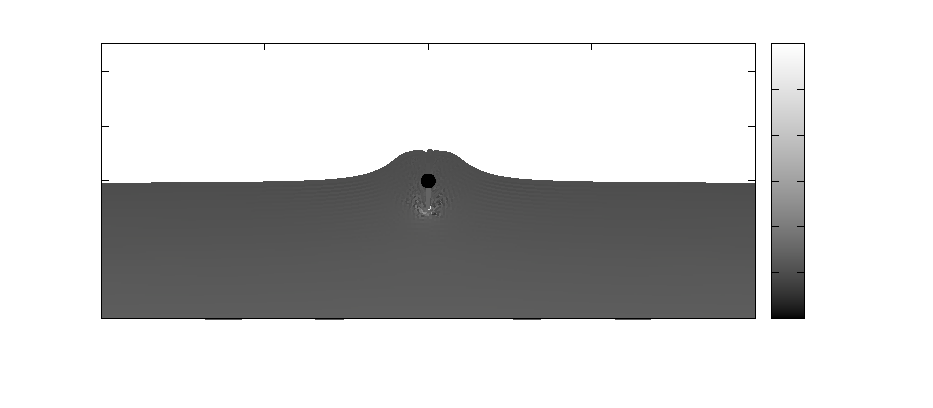
\includegraphics{./4Simulation/Sim200}}%
    \gplfronttext
  \end{picture}%
\endgroup

\caption{$\tau = 0$}
\end{subfigure} \\
\begin{subfigure}{\textwidth}
% GNUPLOT: LaTeX picture with Postscript
\begingroup
  \makeatletter
  \providecommand\color[2][]{%
    \GenericError{(gnuplot) \space\space\space\@spaces}{%
      Package color not loaded in conjunction with
      terminal option `colourtext'%
    }{See the gnuplot documentation for explanation.%
    }{Either use 'blacktext' in gnuplot or load the package
      color.sty in LaTeX.}%
    \renewcommand\color[2][]{}%
  }%
  \providecommand\includegraphics[2][]{%
    \GenericError{(gnuplot) \space\space\space\@spaces}{%
      Package graphicx or graphics not loaded%
    }{See the gnuplot documentation for explanation.%
    }{The gnuplot epslatex terminal needs graphicx.sty or graphics.sty.}%
    \renewcommand\includegraphics[2][]{}%
  }%
  \providecommand\rotatebox[2]{#2}%
  \@ifundefined{ifGPcolor}{%
    \newif\ifGPcolor
    \GPcolorfalse
  }{}%
  \@ifundefined{ifGPblacktext}{%
    \newif\ifGPblacktext
    \GPblacktexttrue
  }{}%
  % define a \g@addto@macro without @ in the name:
  \let\gplgaddtomacro\g@addto@macro
  % define empty templates for all commands taking text:
  \gdef\gplbacktext{}%
  \gdef\gplfronttext{}%
  \makeatother
  \ifGPblacktext
    % no textcolor at all
    \def\colorrgb#1{}%
    \def\colorgray#1{}%
  \else
    % gray or color?
    \ifGPcolor
      \def\colorrgb#1{\color[rgb]{#1}}%
      \def\colorgray#1{\color[gray]{#1}}%
      \expandafter\def\csname LTw\endcsname{\color{white}}%
      \expandafter\def\csname LTb\endcsname{\color{black}}%
      \expandafter\def\csname LTa\endcsname{\color{black}}%
      \expandafter\def\csname LT0\endcsname{\color[rgb]{1,0,0}}%
      \expandafter\def\csname LT1\endcsname{\color[rgb]{0,1,0}}%
      \expandafter\def\csname LT2\endcsname{\color[rgb]{0,0,1}}%
      \expandafter\def\csname LT3\endcsname{\color[rgb]{1,0,1}}%
      \expandafter\def\csname LT4\endcsname{\color[rgb]{0,1,1}}%
      \expandafter\def\csname LT5\endcsname{\color[rgb]{1,1,0}}%
      \expandafter\def\csname LT6\endcsname{\color[rgb]{0,0,0}}%
      \expandafter\def\csname LT7\endcsname{\color[rgb]{1,0.3,0}}%
      \expandafter\def\csname LT8\endcsname{\color[rgb]{0.5,0.5,0.5}}%
    \else
      % gray
      \def\colorrgb#1{\color{black}}%
      \def\colorgray#1{\color[gray]{#1}}%
      \expandafter\def\csname LTw\endcsname{\color{white}}%
      \expandafter\def\csname LTb\endcsname{\color{black}}%
      \expandafter\def\csname LTa\endcsname{\color{black}}%
      \expandafter\def\csname LT0\endcsname{\color{black}}%
      \expandafter\def\csname LT1\endcsname{\color{black}}%
      \expandafter\def\csname LT2\endcsname{\color{black}}%
      \expandafter\def\csname LT3\endcsname{\color{black}}%
      \expandafter\def\csname LT4\endcsname{\color{black}}%
      \expandafter\def\csname LT5\endcsname{\color{black}}%
      \expandafter\def\csname LT6\endcsname{\color{black}}%
      \expandafter\def\csname LT7\endcsname{\color{black}}%
      \expandafter\def\csname LT8\endcsname{\color{black}}%
    \fi
  \fi
    \setlength{\unitlength}{0.0500bp}%
    \ifx\gptboxheight\undefined%
      \newlength{\gptboxheight}%
      \newlength{\gptboxwidth}%
      \newsavebox{\gptboxtext}%
    \fi%
    \setlength{\fboxrule}{0.5pt}%
    \setlength{\fboxsep}{1pt}%
\begin{picture}(8640.00,3600.00)%
    \gplgaddtomacro\gplbacktext{%
      \csname LTb\endcsname%
      \put(682,967){\makebox(0,0)[r]{\strut{}$-4$}}%
      \put(682,1493){\makebox(0,0)[r]{\strut{}$-2$}}%
      \put(682,2020){\makebox(0,0)[r]{\strut{}$0$}}%
      \put(682,2546){\makebox(0,0)[r]{\strut{}$2$}}%
      \put(682,3072){\makebox(0,0)[r]{\strut{}$4$}}%
      \put(814,484){\makebox(0,0){\strut{}$-10$}}%
      \put(2383,484){\makebox(0,0){\strut{}$-5$}}%
      \put(3952,484){\makebox(0,0){\strut{}$0$}}%
      \put(5521,484){\makebox(0,0){\strut{}$5$}}%
      \put(7090,484){\makebox(0,0){\strut{}$10$}}%
    }%
    \gplgaddtomacro\gplfronttext{%
      \csname LTb\endcsname%
      \put(176,2019){\makebox(0,0){\strut{}$y$}}%
      \put(3952,154){\makebox(0,0){\strut{}$x$}}%
      \csname LTb\endcsname%
      \put(7692,704){\makebox(0,0)[l]{\strut{}$0.99$}}%
      \put(7692,1142){\makebox(0,0)[l]{\strut{}$1$}}%
      \put(7692,1581){\makebox(0,0)[l]{\strut{}$1.01$}}%
      \put(7692,2019){\makebox(0,0)[l]{\strut{}$1.02$}}%
      \put(7692,2458){\makebox(0,0)[l]{\strut{}$1.03$}}%
      \put(7692,2896){\makebox(0,0)[l]{\strut{}$1.04$}}%
      \put(7692,3335){\makebox(0,0)[l]{\strut{}$1.05$}}%
      \put(8286,2019){\makebox(0,0){\strut{} $\rho$}}%
    }%
    \gplbacktext
    \put(0,0){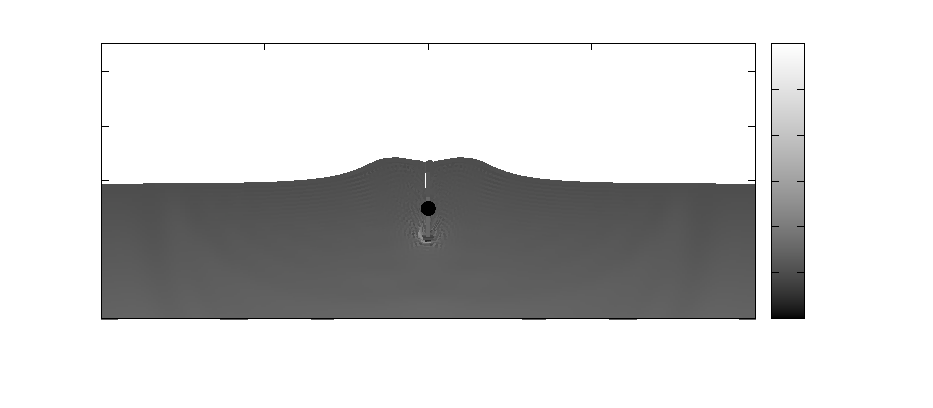
\includegraphics{./Sim201}}%
    \gplfronttext
  \end{picture}%
\endgroup

\caption{$\tau = 1$}
\end{subfigure}
\end{figure}
\begin{figure}[p] \ContinuedFloat
\centering
\begin{subfigure}{\textwidth}
% GNUPLOT: LaTeX picture with Postscript
\begingroup
  \makeatletter
  \providecommand\color[2][]{%
    \GenericError{(gnuplot) \space\space\space\@spaces}{%
      Package color not loaded in conjunction with
      terminal option `colourtext'%
    }{See the gnuplot documentation for explanation.%
    }{Either use 'blacktext' in gnuplot or load the package
      color.sty in LaTeX.}%
    \renewcommand\color[2][]{}%
  }%
  \providecommand\includegraphics[2][]{%
    \GenericError{(gnuplot) \space\space\space\@spaces}{%
      Package graphicx or graphics not loaded%
    }{See the gnuplot documentation for explanation.%
    }{The gnuplot epslatex terminal needs graphicx.sty or graphics.sty.}%
    \renewcommand\includegraphics[2][]{}%
  }%
  \providecommand\rotatebox[2]{#2}%
  \@ifundefined{ifGPcolor}{%
    \newif\ifGPcolor
    \GPcolorfalse
  }{}%
  \@ifundefined{ifGPblacktext}{%
    \newif\ifGPblacktext
    \GPblacktexttrue
  }{}%
  % define a \g@addto@macro without @ in the name:
  \let\gplgaddtomacro\g@addto@macro
  % define empty templates for all commands taking text:
  \gdef\gplbacktext{}%
  \gdef\gplfronttext{}%
  \makeatother
  \ifGPblacktext
    % no textcolor at all
    \def\colorrgb#1{}%
    \def\colorgray#1{}%
  \else
    % gray or color?
    \ifGPcolor
      \def\colorrgb#1{\color[rgb]{#1}}%
      \def\colorgray#1{\color[gray]{#1}}%
      \expandafter\def\csname LTw\endcsname{\color{white}}%
      \expandafter\def\csname LTb\endcsname{\color{black}}%
      \expandafter\def\csname LTa\endcsname{\color{black}}%
      \expandafter\def\csname LT0\endcsname{\color[rgb]{1,0,0}}%
      \expandafter\def\csname LT1\endcsname{\color[rgb]{0,1,0}}%
      \expandafter\def\csname LT2\endcsname{\color[rgb]{0,0,1}}%
      \expandafter\def\csname LT3\endcsname{\color[rgb]{1,0,1}}%
      \expandafter\def\csname LT4\endcsname{\color[rgb]{0,1,1}}%
      \expandafter\def\csname LT5\endcsname{\color[rgb]{1,1,0}}%
      \expandafter\def\csname LT6\endcsname{\color[rgb]{0,0,0}}%
      \expandafter\def\csname LT7\endcsname{\color[rgb]{1,0.3,0}}%
      \expandafter\def\csname LT8\endcsname{\color[rgb]{0.5,0.5,0.5}}%
    \else
      % gray
      \def\colorrgb#1{\color{black}}%
      \def\colorgray#1{\color[gray]{#1}}%
      \expandafter\def\csname LTw\endcsname{\color{white}}%
      \expandafter\def\csname LTb\endcsname{\color{black}}%
      \expandafter\def\csname LTa\endcsname{\color{black}}%
      \expandafter\def\csname LT0\endcsname{\color{black}}%
      \expandafter\def\csname LT1\endcsname{\color{black}}%
      \expandafter\def\csname LT2\endcsname{\color{black}}%
      \expandafter\def\csname LT3\endcsname{\color{black}}%
      \expandafter\def\csname LT4\endcsname{\color{black}}%
      \expandafter\def\csname LT5\endcsname{\color{black}}%
      \expandafter\def\csname LT6\endcsname{\color{black}}%
      \expandafter\def\csname LT7\endcsname{\color{black}}%
      \expandafter\def\csname LT8\endcsname{\color{black}}%
    \fi
  \fi
    \setlength{\unitlength}{0.0500bp}%
    \ifx\gptboxheight\undefined%
      \newlength{\gptboxheight}%
      \newlength{\gptboxwidth}%
      \newsavebox{\gptboxtext}%
    \fi%
    \setlength{\fboxrule}{0.5pt}%
    \setlength{\fboxsep}{1pt}%
\begin{picture}(8640.00,3600.00)%
    \gplgaddtomacro\gplbacktext{%
      \csname LTb\endcsname%
      \put(682,967){\makebox(0,0)[r]{\strut{}$-4$}}%
      \put(682,1493){\makebox(0,0)[r]{\strut{}$-2$}}%
      \put(682,2020){\makebox(0,0)[r]{\strut{}$0$}}%
      \put(682,2546){\makebox(0,0)[r]{\strut{}$2$}}%
      \put(682,3072){\makebox(0,0)[r]{\strut{}$4$}}%
      \put(814,484){\makebox(0,0){\strut{}$-10$}}%
      \put(2383,484){\makebox(0,0){\strut{}$-5$}}%
      \put(3952,484){\makebox(0,0){\strut{}$0$}}%
      \put(5521,484){\makebox(0,0){\strut{}$5$}}%
      \put(7090,484){\makebox(0,0){\strut{}$10$}}%
    }%
    \gplgaddtomacro\gplfronttext{%
      \csname LTb\endcsname%
      \put(176,2019){\makebox(0,0){\strut{}$y$}}%
      \put(3952,154){\makebox(0,0){\strut{}$x$}}%
      \csname LTb\endcsname%
      \put(7692,704){\makebox(0,0)[l]{\strut{}$0.99$}}%
      \put(7692,1142){\makebox(0,0)[l]{\strut{}$1$}}%
      \put(7692,1581){\makebox(0,0)[l]{\strut{}$1.01$}}%
      \put(7692,2019){\makebox(0,0)[l]{\strut{}$1.02$}}%
      \put(7692,2458){\makebox(0,0)[l]{\strut{}$1.03$}}%
      \put(7692,2896){\makebox(0,0)[l]{\strut{}$1.04$}}%
      \put(7692,3335){\makebox(0,0)[l]{\strut{}$1.05$}}%
      \put(8286,2019){\makebox(0,0){\strut{} $\rho$}}%
    }%
    \gplbacktext
    \put(0,0){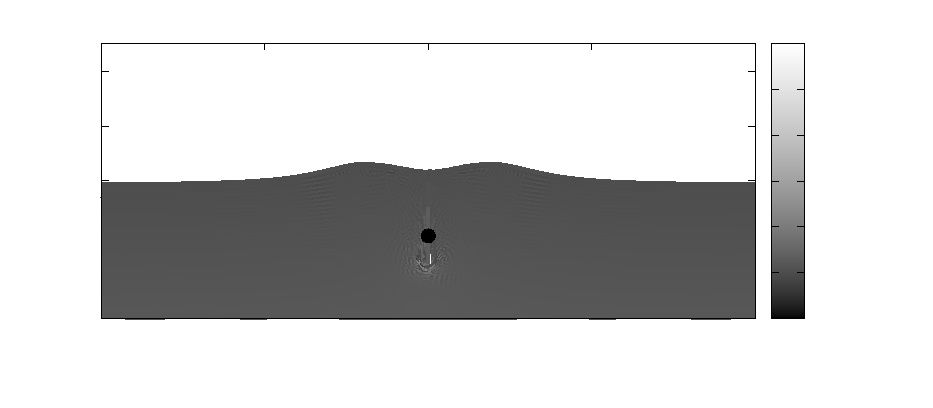
\includegraphics{./Sim202}}%
    \gplfronttext
  \end{picture}%
\endgroup

\caption{$\tau = 2$}
\end{subfigure} \\
\begin{subfigure}{\textwidth}
% GNUPLOT: LaTeX picture with Postscript
\begingroup
  \makeatletter
  \providecommand\color[2][]{%
    \GenericError{(gnuplot) \space\space\space\@spaces}{%
      Package color not loaded in conjunction with
      terminal option `colourtext'%
    }{See the gnuplot documentation for explanation.%
    }{Either use 'blacktext' in gnuplot or load the package
      color.sty in LaTeX.}%
    \renewcommand\color[2][]{}%
  }%
  \providecommand\includegraphics[2][]{%
    \GenericError{(gnuplot) \space\space\space\@spaces}{%
      Package graphicx or graphics not loaded%
    }{See the gnuplot documentation for explanation.%
    }{The gnuplot epslatex terminal needs graphicx.sty or graphics.sty.}%
    \renewcommand\includegraphics[2][]{}%
  }%
  \providecommand\rotatebox[2]{#2}%
  \@ifundefined{ifGPcolor}{%
    \newif\ifGPcolor
    \GPcolorfalse
  }{}%
  \@ifundefined{ifGPblacktext}{%
    \newif\ifGPblacktext
    \GPblacktexttrue
  }{}%
  % define a \g@addto@macro without @ in the name:
  \let\gplgaddtomacro\g@addto@macro
  % define empty templates for all commands taking text:
  \gdef\gplbacktext{}%
  \gdef\gplfronttext{}%
  \makeatother
  \ifGPblacktext
    % no textcolor at all
    \def\colorrgb#1{}%
    \def\colorgray#1{}%
  \else
    % gray or color?
    \ifGPcolor
      \def\colorrgb#1{\color[rgb]{#1}}%
      \def\colorgray#1{\color[gray]{#1}}%
      \expandafter\def\csname LTw\endcsname{\color{white}}%
      \expandafter\def\csname LTb\endcsname{\color{black}}%
      \expandafter\def\csname LTa\endcsname{\color{black}}%
      \expandafter\def\csname LT0\endcsname{\color[rgb]{1,0,0}}%
      \expandafter\def\csname LT1\endcsname{\color[rgb]{0,1,0}}%
      \expandafter\def\csname LT2\endcsname{\color[rgb]{0,0,1}}%
      \expandafter\def\csname LT3\endcsname{\color[rgb]{1,0,1}}%
      \expandafter\def\csname LT4\endcsname{\color[rgb]{0,1,1}}%
      \expandafter\def\csname LT5\endcsname{\color[rgb]{1,1,0}}%
      \expandafter\def\csname LT6\endcsname{\color[rgb]{0,0,0}}%
      \expandafter\def\csname LT7\endcsname{\color[rgb]{1,0.3,0}}%
      \expandafter\def\csname LT8\endcsname{\color[rgb]{0.5,0.5,0.5}}%
    \else
      % gray
      \def\colorrgb#1{\color{black}}%
      \def\colorgray#1{\color[gray]{#1}}%
      \expandafter\def\csname LTw\endcsname{\color{white}}%
      \expandafter\def\csname LTb\endcsname{\color{black}}%
      \expandafter\def\csname LTa\endcsname{\color{black}}%
      \expandafter\def\csname LT0\endcsname{\color{black}}%
      \expandafter\def\csname LT1\endcsname{\color{black}}%
      \expandafter\def\csname LT2\endcsname{\color{black}}%
      \expandafter\def\csname LT3\endcsname{\color{black}}%
      \expandafter\def\csname LT4\endcsname{\color{black}}%
      \expandafter\def\csname LT5\endcsname{\color{black}}%
      \expandafter\def\csname LT6\endcsname{\color{black}}%
      \expandafter\def\csname LT7\endcsname{\color{black}}%
      \expandafter\def\csname LT8\endcsname{\color{black}}%
    \fi
  \fi
    \setlength{\unitlength}{0.0500bp}%
    \ifx\gptboxheight\undefined%
      \newlength{\gptboxheight}%
      \newlength{\gptboxwidth}%
      \newsavebox{\gptboxtext}%
    \fi%
    \setlength{\fboxrule}{0.5pt}%
    \setlength{\fboxsep}{1pt}%
\begin{picture}(8640.00,3600.00)%
    \gplgaddtomacro\gplbacktext{%
      \csname LTb\endcsname%
      \put(682,967){\makebox(0,0)[r]{\strut{}$-4$}}%
      \put(682,1493){\makebox(0,0)[r]{\strut{}$-2$}}%
      \put(682,2020){\makebox(0,0)[r]{\strut{}$0$}}%
      \put(682,2546){\makebox(0,0)[r]{\strut{}$2$}}%
      \put(682,3072){\makebox(0,0)[r]{\strut{}$4$}}%
      \put(814,484){\makebox(0,0){\strut{}$-10$}}%
      \put(2383,484){\makebox(0,0){\strut{}$-5$}}%
      \put(3952,484){\makebox(0,0){\strut{}$0$}}%
      \put(5521,484){\makebox(0,0){\strut{}$5$}}%
      \put(7090,484){\makebox(0,0){\strut{}$10$}}%
    }%
    \gplgaddtomacro\gplfronttext{%
      \csname LTb\endcsname%
      \put(176,2019){\makebox(0,0){\strut{}$y$}}%
      \put(3952,154){\makebox(0,0){\strut{}$x$}}%
      \csname LTb\endcsname%
      \put(7692,704){\makebox(0,0)[l]{\strut{}$0.99$}}%
      \put(7692,1142){\makebox(0,0)[l]{\strut{}$1$}}%
      \put(7692,1581){\makebox(0,0)[l]{\strut{}$1.01$}}%
      \put(7692,2019){\makebox(0,0)[l]{\strut{}$1.02$}}%
      \put(7692,2458){\makebox(0,0)[l]{\strut{}$1.03$}}%
      \put(7692,2896){\makebox(0,0)[l]{\strut{}$1.04$}}%
      \put(7692,3335){\makebox(0,0)[l]{\strut{}$1.05$}}%
      \put(8286,2019){\makebox(0,0){\strut{} $\rho$}}%
    }%
    \gplbacktext
    \put(0,0){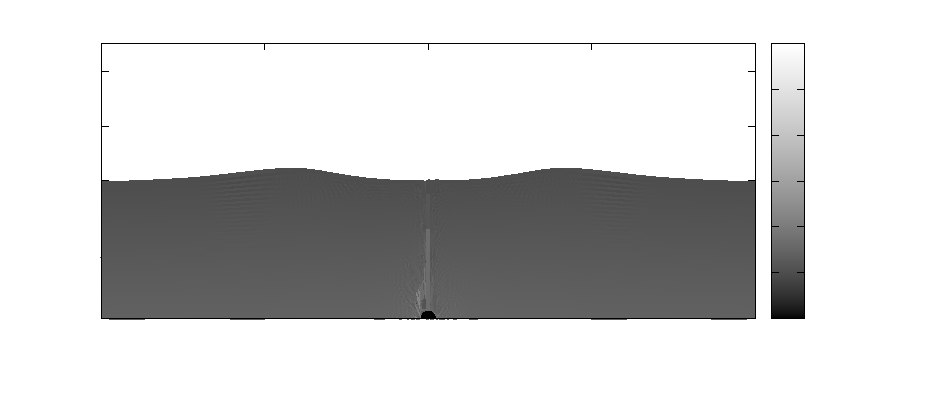
\includegraphics{./4Simulation/Sim205}}%
    \gplfronttext
  \end{picture}%
\endgroup

\caption{$\tau = 5$}
\end{subfigure} \\
\begin{subfigure}{\textwidth}
% GNUPLOT: LaTeX picture with Postscript
\begingroup
  \makeatletter
  \providecommand\color[2][]{%
    \GenericError{(gnuplot) \space\space\space\@spaces}{%
      Package color not loaded in conjunction with
      terminal option `colourtext'%
    }{See the gnuplot documentation for explanation.%
    }{Either use 'blacktext' in gnuplot or load the package
      color.sty in LaTeX.}%
    \renewcommand\color[2][]{}%
  }%
  \providecommand\includegraphics[2][]{%
    \GenericError{(gnuplot) \space\space\space\@spaces}{%
      Package graphicx or graphics not loaded%
    }{See the gnuplot documentation for explanation.%
    }{The gnuplot epslatex terminal needs graphicx.sty or graphics.sty.}%
    \renewcommand\includegraphics[2][]{}%
  }%
  \providecommand\rotatebox[2]{#2}%
  \@ifundefined{ifGPcolor}{%
    \newif\ifGPcolor
    \GPcolorfalse
  }{}%
  \@ifundefined{ifGPblacktext}{%
    \newif\ifGPblacktext
    \GPblacktexttrue
  }{}%
  % define a \g@addto@macro without @ in the name:
  \let\gplgaddtomacro\g@addto@macro
  % define empty templates for all commands taking text:
  \gdef\gplbacktext{}%
  \gdef\gplfronttext{}%
  \makeatother
  \ifGPblacktext
    % no textcolor at all
    \def\colorrgb#1{}%
    \def\colorgray#1{}%
  \else
    % gray or color?
    \ifGPcolor
      \def\colorrgb#1{\color[rgb]{#1}}%
      \def\colorgray#1{\color[gray]{#1}}%
      \expandafter\def\csname LTw\endcsname{\color{white}}%
      \expandafter\def\csname LTb\endcsname{\color{black}}%
      \expandafter\def\csname LTa\endcsname{\color{black}}%
      \expandafter\def\csname LT0\endcsname{\color[rgb]{1,0,0}}%
      \expandafter\def\csname LT1\endcsname{\color[rgb]{0,1,0}}%
      \expandafter\def\csname LT2\endcsname{\color[rgb]{0,0,1}}%
      \expandafter\def\csname LT3\endcsname{\color[rgb]{1,0,1}}%
      \expandafter\def\csname LT4\endcsname{\color[rgb]{0,1,1}}%
      \expandafter\def\csname LT5\endcsname{\color[rgb]{1,1,0}}%
      \expandafter\def\csname LT6\endcsname{\color[rgb]{0,0,0}}%
      \expandafter\def\csname LT7\endcsname{\color[rgb]{1,0.3,0}}%
      \expandafter\def\csname LT8\endcsname{\color[rgb]{0.5,0.5,0.5}}%
    \else
      % gray
      \def\colorrgb#1{\color{black}}%
      \def\colorgray#1{\color[gray]{#1}}%
      \expandafter\def\csname LTw\endcsname{\color{white}}%
      \expandafter\def\csname LTb\endcsname{\color{black}}%
      \expandafter\def\csname LTa\endcsname{\color{black}}%
      \expandafter\def\csname LT0\endcsname{\color{black}}%
      \expandafter\def\csname LT1\endcsname{\color{black}}%
      \expandafter\def\csname LT2\endcsname{\color{black}}%
      \expandafter\def\csname LT3\endcsname{\color{black}}%
      \expandafter\def\csname LT4\endcsname{\color{black}}%
      \expandafter\def\csname LT5\endcsname{\color{black}}%
      \expandafter\def\csname LT6\endcsname{\color{black}}%
      \expandafter\def\csname LT7\endcsname{\color{black}}%
      \expandafter\def\csname LT8\endcsname{\color{black}}%
    \fi
  \fi
    \setlength{\unitlength}{0.0500bp}%
    \ifx\gptboxheight\undefined%
      \newlength{\gptboxheight}%
      \newlength{\gptboxwidth}%
      \newsavebox{\gptboxtext}%
    \fi%
    \setlength{\fboxrule}{0.5pt}%
    \setlength{\fboxsep}{1pt}%
\begin{picture}(8640.00,3600.00)%
    \gplgaddtomacro\gplbacktext{%
      \csname LTb\endcsname%
      \put(682,967){\makebox(0,0)[r]{\strut{}$-4$}}%
      \put(682,1493){\makebox(0,0)[r]{\strut{}$-2$}}%
      \put(682,2020){\makebox(0,0)[r]{\strut{}$0$}}%
      \put(682,2546){\makebox(0,0)[r]{\strut{}$2$}}%
      \put(682,3072){\makebox(0,0)[r]{\strut{}$4$}}%
      \put(814,484){\makebox(0,0){\strut{}$-10$}}%
      \put(2383,484){\makebox(0,0){\strut{}$-5$}}%
      \put(3952,484){\makebox(0,0){\strut{}$0$}}%
      \put(5521,484){\makebox(0,0){\strut{}$5$}}%
      \put(7090,484){\makebox(0,0){\strut{}$10$}}%
    }%
    \gplgaddtomacro\gplfronttext{%
      \csname LTb\endcsname%
      \put(176,2019){\makebox(0,0){\strut{}$y$}}%
      \put(3952,154){\makebox(0,0){\strut{}$x$}}%
      \csname LTb\endcsname%
      \put(7692,704){\makebox(0,0)[l]{\strut{}$0.99$}}%
      \put(7692,1142){\makebox(0,0)[l]{\strut{}$1$}}%
      \put(7692,1581){\makebox(0,0)[l]{\strut{}$1.01$}}%
      \put(7692,2019){\makebox(0,0)[l]{\strut{}$1.02$}}%
      \put(7692,2458){\makebox(0,0)[l]{\strut{}$1.03$}}%
      \put(7692,2896){\makebox(0,0)[l]{\strut{}$1.04$}}%
      \put(7692,3335){\makebox(0,0)[l]{\strut{}$1.05$}}%
      \put(8286,2019){\makebox(0,0){\strut{} $\rho$}}%
    }%
    \gplbacktext
    \put(0,0){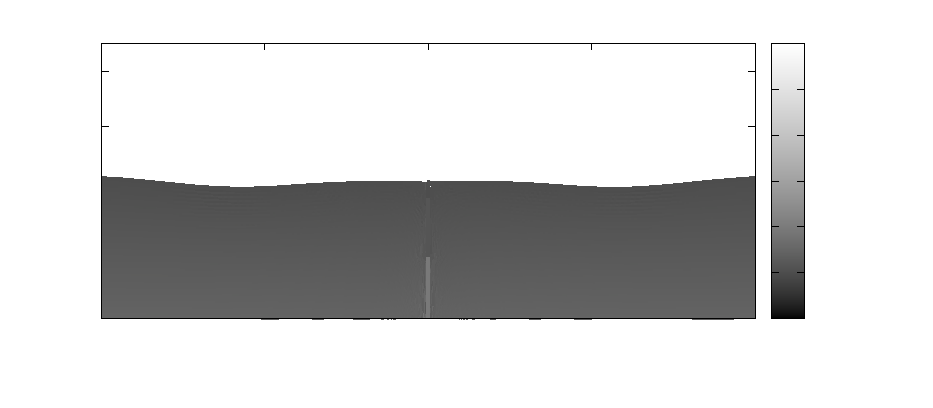
\includegraphics{./Sim210}}%
    \gplfronttext
  \end{picture}%
\endgroup

\caption{$\tau = 10$}
\end{subfigure}
\caption[Surface waves resulting from the simulation]{Surface waves resulting from the simulation.  The full animation can be found at \url{https://github.com/bmetherall/Primordial_Black_Holes/blob/master/Videos/Simulation.gif}.}
\label{fig:simresults}
\end{figure}
As with the analytic results, we see that the surface of the neutron star pulls upwards before the collision due to the gravitational force of the primordial black hole. Then, after the collision, the initial wave propagates outwards. It is fairly difficult to notice, however, a second much smaller amplitude wave is created as well. Unfortunately, because of the resolution of the simulation, waves smaller than $dx$ cannot be seen, unlike in the analytic solution which had a much smaller spacing. \\

In order to calculate the energy we do so in the traditional way, by taking the sum of the potential and kinetic energies of each particle,
\begin{align*}
E &= \sum_i T_i + U_i, \\
&= \sum_i \frac{1}{2} m_i \left( u_i^2 + v_i^2 \right) + m_i g y_i.
\end{align*}
However, to compare to the analytic result, we must transform this into three dimensions by revolving about the $y$ axis. This can be done by weighting each particle by $\pi |x_i| / dx$,
\begin{align*}
E &= \frac{\pi}{dx} \sum_i \left( \frac{1}{2} \left( u_i^2 + v_i^2 \right) + g y_i \right) m_i |x_i|.
\end{align*}

\begin{figure}
\centering
\begin{subfigure}{\textwidth}
% GNUPLOT: LaTeX picture with Postscript
\begingroup
  \makeatletter
  \providecommand\color[2][]{%
    \GenericError{(gnuplot) \space\space\space\@spaces}{%
      Package color not loaded in conjunction with
      terminal option `colourtext'%
    }{See the gnuplot documentation for explanation.%
    }{Either use 'blacktext' in gnuplot or load the package
      color.sty in LaTeX.}%
    \renewcommand\color[2][]{}%
  }%
  \providecommand\includegraphics[2][]{%
    \GenericError{(gnuplot) \space\space\space\@spaces}{%
      Package graphicx or graphics not loaded%
    }{See the gnuplot documentation for explanation.%
    }{The gnuplot epslatex terminal needs graphicx.sty or graphics.sty.}%
    \renewcommand\includegraphics[2][]{}%
  }%
  \providecommand\rotatebox[2]{#2}%
  \@ifundefined{ifGPcolor}{%
    \newif\ifGPcolor
    \GPcolorfalse
  }{}%
  \@ifundefined{ifGPblacktext}{%
    \newif\ifGPblacktext
    \GPblacktexttrue
  }{}%
  % define a \g@addto@macro without @ in the name:
  \let\gplgaddtomacro\g@addto@macro
  % define empty templates for all commands taking text:
  \gdef\gplbacktext{}%
  \gdef\gplfronttext{}%
  \makeatother
  \ifGPblacktext
    % no textcolor at all
    \def\colorrgb#1{}%
    \def\colorgray#1{}%
  \else
    % gray or color?
    \ifGPcolor
      \def\colorrgb#1{\color[rgb]{#1}}%
      \def\colorgray#1{\color[gray]{#1}}%
      \expandafter\def\csname LTw\endcsname{\color{white}}%
      \expandafter\def\csname LTb\endcsname{\color{black}}%
      \expandafter\def\csname LTa\endcsname{\color{black}}%
      \expandafter\def\csname LT0\endcsname{\color[rgb]{1,0,0}}%
      \expandafter\def\csname LT1\endcsname{\color[rgb]{0,1,0}}%
      \expandafter\def\csname LT2\endcsname{\color[rgb]{0,0,1}}%
      \expandafter\def\csname LT3\endcsname{\color[rgb]{1,0,1}}%
      \expandafter\def\csname LT4\endcsname{\color[rgb]{0,1,1}}%
      \expandafter\def\csname LT5\endcsname{\color[rgb]{1,1,0}}%
      \expandafter\def\csname LT6\endcsname{\color[rgb]{0,0,0}}%
      \expandafter\def\csname LT7\endcsname{\color[rgb]{1,0.3,0}}%
      \expandafter\def\csname LT8\endcsname{\color[rgb]{0.5,0.5,0.5}}%
    \else
      % gray
      \def\colorrgb#1{\color{black}}%
      \def\colorgray#1{\color[gray]{#1}}%
      \expandafter\def\csname LTw\endcsname{\color{white}}%
      \expandafter\def\csname LTb\endcsname{\color{black}}%
      \expandafter\def\csname LTa\endcsname{\color{black}}%
      \expandafter\def\csname LT0\endcsname{\color{black}}%
      \expandafter\def\csname LT1\endcsname{\color{black}}%
      \expandafter\def\csname LT2\endcsname{\color{black}}%
      \expandafter\def\csname LT3\endcsname{\color{black}}%
      \expandafter\def\csname LT4\endcsname{\color{black}}%
      \expandafter\def\csname LT5\endcsname{\color{black}}%
      \expandafter\def\csname LT6\endcsname{\color{black}}%
      \expandafter\def\csname LT7\endcsname{\color{black}}%
      \expandafter\def\csname LT8\endcsname{\color{black}}%
    \fi
  \fi
    \setlength{\unitlength}{0.0500bp}%
    \ifx\gptboxheight\undefined%
      \newlength{\gptboxheight}%
      \newlength{\gptboxwidth}%
      \newsavebox{\gptboxtext}%
    \fi%
    \setlength{\fboxrule}{0.5pt}%
    \setlength{\fboxsep}{1pt}%
\begin{picture}(8640.00,5400.00)%
    \gplgaddtomacro\gplbacktext{%
      \csname LTb\endcsname%
      \put(1606,704){\makebox(0,0)[r]{\strut{}$5.42\times10^{6}$}}%
      \csname LTb\endcsname%
      \put(1606,1337){\makebox(0,0)[r]{\strut{}$5.425\times10^{6}$}}%
      \csname LTb\endcsname%
      \put(1606,1970){\makebox(0,0)[r]{\strut{}$5.43\times10^{6}$}}%
      \csname LTb\endcsname%
      \put(1606,2603){\makebox(0,0)[r]{\strut{}$5.435\times10^{6}$}}%
      \csname LTb\endcsname%
      \put(1606,3236){\makebox(0,0)[r]{\strut{}$5.44\times10^{6}$}}%
      \csname LTb\endcsname%
      \put(1606,3869){\makebox(0,0)[r]{\strut{}$5.445\times10^{6}$}}%
      \csname LTb\endcsname%
      \put(1606,4502){\makebox(0,0)[r]{\strut{}$5.45\times10^{6}$}}%
      \csname LTb\endcsname%
      \put(1606,5135){\makebox(0,0)[r]{\strut{}$5.455\times10^{6}$}}%
      \csname LTb\endcsname%
      \put(2099,484){\makebox(0,0){\strut{}$-80$}}%
      \csname LTb\endcsname%
      \put(2822,484){\makebox(0,0){\strut{}$-60$}}%
      \csname LTb\endcsname%
      \put(3545,484){\makebox(0,0){\strut{}$-40$}}%
      \csname LTb\endcsname%
      \put(4268,484){\makebox(0,0){\strut{}$-20$}}%
      \csname LTb\endcsname%
      \put(4991,484){\makebox(0,0){\strut{}$0$}}%
      \csname LTb\endcsname%
      \put(5713,484){\makebox(0,0){\strut{}$20$}}%
      \csname LTb\endcsname%
      \put(6436,484){\makebox(0,0){\strut{}$40$}}%
      \csname LTb\endcsname%
      \put(7159,484){\makebox(0,0){\strut{}$60$}}%
      \csname LTb\endcsname%
      \put(7882,484){\makebox(0,0){\strut{}$80$}}%
    }%
    \gplgaddtomacro\gplfronttext{%
      \csname LTb\endcsname%
      \put(176,2919){\makebox(0,0){\strut{}$E$}}%
      \put(4990,154){\makebox(0,0){\strut{}$\tau$}}%
    }%
    \gplbacktext
    \put(0,0){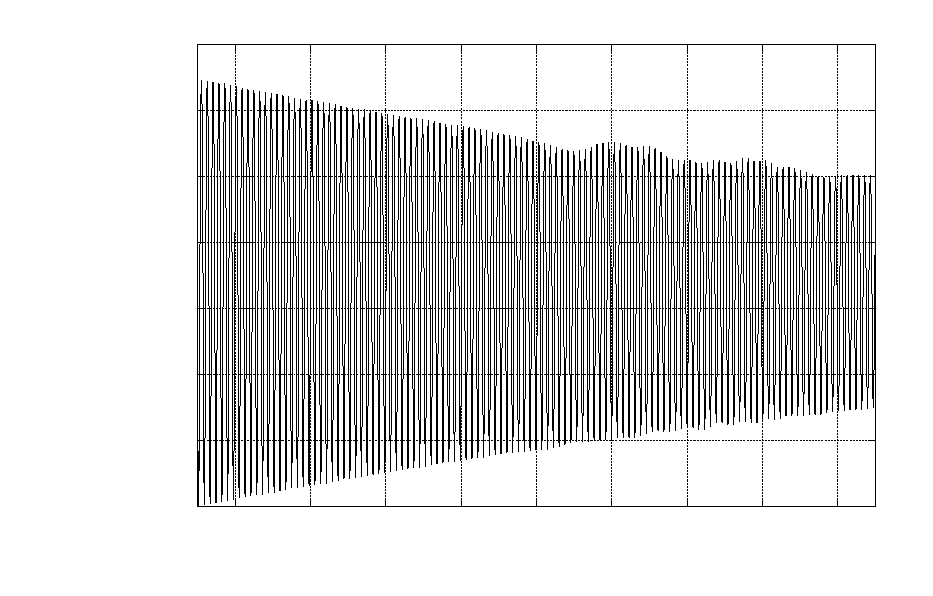
\includegraphics{BadEnergy}}%
    \gplfronttext
  \end{picture}%
\endgroup

\caption{Crazy looking energy.}
\label{fig:badenergy}
\end{subfigure} \\
\begin{subfigure}{\textwidth}
% GNUPLOT: LaTeX picture with Postscript
\begingroup
  \makeatletter
  \providecommand\color[2][]{%
    \GenericError{(gnuplot) \space\space\space\@spaces}{%
      Package color not loaded in conjunction with
      terminal option `colourtext'%
    }{See the gnuplot documentation for explanation.%
    }{Either use 'blacktext' in gnuplot or load the package
      color.sty in LaTeX.}%
    \renewcommand\color[2][]{}%
  }%
  \providecommand\includegraphics[2][]{%
    \GenericError{(gnuplot) \space\space\space\@spaces}{%
      Package graphicx or graphics not loaded%
    }{See the gnuplot documentation for explanation.%
    }{The gnuplot epslatex terminal needs graphicx.sty or graphics.sty.}%
    \renewcommand\includegraphics[2][]{}%
  }%
  \providecommand\rotatebox[2]{#2}%
  \@ifundefined{ifGPcolor}{%
    \newif\ifGPcolor
    \GPcolortrue
  }{}%
  \@ifundefined{ifGPblacktext}{%
    \newif\ifGPblacktext
    \GPblacktexttrue
  }{}%
  % define a \g@addto@macro without @ in the name:
  \let\gplgaddtomacro\g@addto@macro
  % define empty templates for all commands taking text:
  \gdef\gplbacktext{}%
  \gdef\gplfronttext{}%
  \makeatother
  \ifGPblacktext
    % no textcolor at all
    \def\colorrgb#1{}%
    \def\colorgray#1{}%
  \else
    % gray or color?
    \ifGPcolor
      \def\colorrgb#1{\color[rgb]{#1}}%
      \def\colorgray#1{\color[gray]{#1}}%
      \expandafter\def\csname LTw\endcsname{\color{white}}%
      \expandafter\def\csname LTb\endcsname{\color{black}}%
      \expandafter\def\csname LTa\endcsname{\color{black}}%
      \expandafter\def\csname LT0\endcsname{\color[rgb]{1,0,0}}%
      \expandafter\def\csname LT1\endcsname{\color[rgb]{0,1,0}}%
      \expandafter\def\csname LT2\endcsname{\color[rgb]{0,0,1}}%
      \expandafter\def\csname LT3\endcsname{\color[rgb]{1,0,1}}%
      \expandafter\def\csname LT4\endcsname{\color[rgb]{0,1,1}}%
      \expandafter\def\csname LT5\endcsname{\color[rgb]{1,1,0}}%
      \expandafter\def\csname LT6\endcsname{\color[rgb]{0,0,0}}%
      \expandafter\def\csname LT7\endcsname{\color[rgb]{1,0.3,0}}%
      \expandafter\def\csname LT8\endcsname{\color[rgb]{0.5,0.5,0.5}}%
    \else
      % gray
      \def\colorrgb#1{\color{black}}%
      \def\colorgray#1{\color[gray]{#1}}%
      \expandafter\def\csname LTw\endcsname{\color{white}}%
      \expandafter\def\csname LTb\endcsname{\color{black}}%
      \expandafter\def\csname LTa\endcsname{\color{black}}%
      \expandafter\def\csname LT0\endcsname{\color{black}}%
      \expandafter\def\csname LT1\endcsname{\color{black}}%
      \expandafter\def\csname LT2\endcsname{\color{black}}%
      \expandafter\def\csname LT3\endcsname{\color{black}}%
      \expandafter\def\csname LT4\endcsname{\color{black}}%
      \expandafter\def\csname LT5\endcsname{\color{black}}%
      \expandafter\def\csname LT6\endcsname{\color{black}}%
      \expandafter\def\csname LT7\endcsname{\color{black}}%
      \expandafter\def\csname LT8\endcsname{\color{black}}%
    \fi
  \fi
    \setlength{\unitlength}{0.0500bp}%
    \ifx\gptboxheight\undefined%
      \newlength{\gptboxheight}%
      \newlength{\gptboxwidth}%
      \newsavebox{\gptboxtext}%
    \fi%
    \setlength{\fboxrule}{0.5pt}%
    \setlength{\fboxsep}{1pt}%
\begin{picture}(5760.00,3844.00)%
    \gplgaddtomacro\gplbacktext{%
      \csname LTb\endcsname%
      \put(946,704){\makebox(0,0)[r]{\strut{}$-200$}}%
      \csname LTb\endcsname%
      \put(946,1023){\makebox(0,0)[r]{\strut{}$0$}}%
      \csname LTb\endcsname%
      \put(946,1343){\makebox(0,0)[r]{\strut{}$200$}}%
      \csname LTb\endcsname%
      \put(946,1662){\makebox(0,0)[r]{\strut{}$400$}}%
      \csname LTb\endcsname%
      \put(946,1982){\makebox(0,0)[r]{\strut{}$600$}}%
      \csname LTb\endcsname%
      \put(946,2301){\makebox(0,0)[r]{\strut{}$800$}}%
      \csname LTb\endcsname%
      \put(946,2621){\makebox(0,0)[r]{\strut{}$1000$}}%
      \csname LTb\endcsname%
      \put(946,2940){\makebox(0,0)[r]{\strut{}$1200$}}%
      \csname LTb\endcsname%
      \put(946,3260){\makebox(0,0)[r]{\strut{}$1400$}}%
      \csname LTb\endcsname%
      \put(946,3579){\makebox(0,0)[r]{\strut{}$1600$}}%
      \csname LTb\endcsname%
      \put(1316,484){\makebox(0,0){\strut{}$-80$}}%
      \csname LTb\endcsname%
      \put(1792,484){\makebox(0,0){\strut{}$-60$}}%
      \csname LTb\endcsname%
      \put(2268,484){\makebox(0,0){\strut{}$-40$}}%
      \csname LTb\endcsname%
      \put(2744,484){\makebox(0,0){\strut{}$-20$}}%
      \csname LTb\endcsname%
      \put(3221,484){\makebox(0,0){\strut{}$0$}}%
      \csname LTb\endcsname%
      \put(3697,484){\makebox(0,0){\strut{}$20$}}%
      \csname LTb\endcsname%
      \put(4173,484){\makebox(0,0){\strut{}$40$}}%
      \csname LTb\endcsname%
      \put(4649,484){\makebox(0,0){\strut{}$60$}}%
      \csname LTb\endcsname%
      \put(5125,484){\makebox(0,0){\strut{}$80$}}%
    }%
    \gplgaddtomacro\gplfronttext{%
      \csname LTb\endcsname%
      \put(176,2141){\rotatebox{-270}{\makebox(0,0){\strut{}$E$}}}%
      \put(3220,154){\makebox(0,0){\strut{}$\tau$}}%
    }%
    \gplbacktext
    \put(0,0){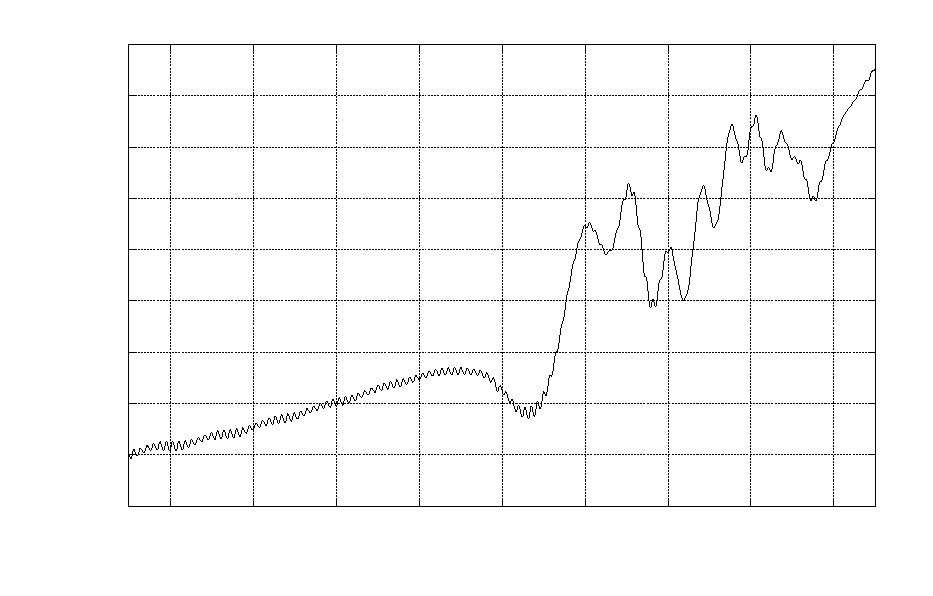
\includegraphics{./GoodEnergy}}%
    \gplfronttext
  \end{picture}%
\endgroup

\caption{Smoothed energy without noise.}
\label{fig:goodenergy}
\end{subfigure}
\caption{Energy transfer from the simulation.}
\end{figure}

This is essentially the same as a shell integration, however, we only integrate through $\pi$, and the absolute value of the $x$ coordinate is needed. The energy is calculated in this fashion for all time steps and is plotted in Figure \ref{fig:badenergy}. Clearly, this is of little use since the energy is full of noise and highly oscillatory. As mentioned before, this is also the result of how the particles are initially placed within the simulation. As the surface oscillates up and down while attempting to equilibrate, so too does the potential energy. The oscillations have a period of 39 time steps, and therefore, by taking running averages of 39 time steps, most of the noise is removed. Also for clarity, the damping is removed, and the energy has been shifted to start at 0; the resulting plot is much cleaner and is in Figure \ref{fig:goodenergy}. \\

This cleaned up energy has a very similar shape to the analytic calculation; initially, the neutron star gains energy as the primordial black hole approaches. And after the collision there is a large peak in the energy similar to the analytic solution. However, this jump in energy is much larger. Furthermore, at approximately $\tau = 40$ the initial wave hits the boundaries which causes the energy of the system to increase as the wave climbs the wall. After this, the wave is reflected back towards the centre of the tank. This also causes the first wave to interfere with the smaller waves trailing it which again causes the energy to increase -- this is the main cause of the erratic behaviour of the energy at times greater than 40. \\

Another point of interest is that since the tank has a depth of $15$, at $\tau = 15$ the primordial black hole exits the tank. During the lower resolution testing this did not appear to affect the results of the simulation, however, it indeed does. As the primordial black hole exits the tank a shock wave is created. In Figure \ref{fig:shock} the shock wave can be seen moving outwards from the bottom of the tank, and when it reaches the surface, it is reflected back into the star. Given the speed of the shock wave and the dimensions of the tank, it will be dampened out within a few time units and does not appear to effect the energy of the system.

\begin{figure}
\centering
\begin{subfigure}{\textwidth}
% GNUPLOT: LaTeX picture with Postscript
\begingroup
  \makeatletter
  \providecommand\color[2][]{%
    \GenericError{(gnuplot) \space\space\space\@spaces}{%
      Package color not loaded in conjunction with
      terminal option `colourtext'%
    }{See the gnuplot documentation for explanation.%
    }{Either use 'blacktext' in gnuplot or load the package
      color.sty in LaTeX.}%
    \renewcommand\color[2][]{}%
  }%
  \providecommand\includegraphics[2][]{%
    \GenericError{(gnuplot) \space\space\space\@spaces}{%
      Package graphicx or graphics not loaded%
    }{See the gnuplot documentation for explanation.%
    }{The gnuplot epslatex terminal needs graphicx.sty or graphics.sty.}%
    \renewcommand\includegraphics[2][]{}%
  }%
  \providecommand\rotatebox[2]{#2}%
  \@ifundefined{ifGPcolor}{%
    \newif\ifGPcolor
    \GPcolorfalse
  }{}%
  \@ifundefined{ifGPblacktext}{%
    \newif\ifGPblacktext
    \GPblacktexttrue
  }{}%
  % define a \g@addto@macro without @ in the name:
  \let\gplgaddtomacro\g@addto@macro
  % define empty templates for all commands taking text:
  \gdef\gplbacktext{}%
  \gdef\gplfronttext{}%
  \makeatother
  \ifGPblacktext
    % no textcolor at all
    \def\colorrgb#1{}%
    \def\colorgray#1{}%
  \else
    % gray or color?
    \ifGPcolor
      \def\colorrgb#1{\color[rgb]{#1}}%
      \def\colorgray#1{\color[gray]{#1}}%
      \expandafter\def\csname LTw\endcsname{\color{white}}%
      \expandafter\def\csname LTb\endcsname{\color{black}}%
      \expandafter\def\csname LTa\endcsname{\color{black}}%
      \expandafter\def\csname LT0\endcsname{\color[rgb]{1,0,0}}%
      \expandafter\def\csname LT1\endcsname{\color[rgb]{0,1,0}}%
      \expandafter\def\csname LT2\endcsname{\color[rgb]{0,0,1}}%
      \expandafter\def\csname LT3\endcsname{\color[rgb]{1,0,1}}%
      \expandafter\def\csname LT4\endcsname{\color[rgb]{0,1,1}}%
      \expandafter\def\csname LT5\endcsname{\color[rgb]{1,1,0}}%
      \expandafter\def\csname LT6\endcsname{\color[rgb]{0,0,0}}%
      \expandafter\def\csname LT7\endcsname{\color[rgb]{1,0.3,0}}%
      \expandafter\def\csname LT8\endcsname{\color[rgb]{0.5,0.5,0.5}}%
    \else
      % gray
      \def\colorrgb#1{\color{black}}%
      \def\colorgray#1{\color[gray]{#1}}%
      \expandafter\def\csname LTw\endcsname{\color{white}}%
      \expandafter\def\csname LTb\endcsname{\color{black}}%
      \expandafter\def\csname LTa\endcsname{\color{black}}%
      \expandafter\def\csname LT0\endcsname{\color{black}}%
      \expandafter\def\csname LT1\endcsname{\color{black}}%
      \expandafter\def\csname LT2\endcsname{\color{black}}%
      \expandafter\def\csname LT3\endcsname{\color{black}}%
      \expandafter\def\csname LT4\endcsname{\color{black}}%
      \expandafter\def\csname LT5\endcsname{\color{black}}%
      \expandafter\def\csname LT6\endcsname{\color{black}}%
      \expandafter\def\csname LT7\endcsname{\color{black}}%
      \expandafter\def\csname LT8\endcsname{\color{black}}%
    \fi
  \fi
    \setlength{\unitlength}{0.0500bp}%
    \ifx\gptboxheight\undefined%
      \newlength{\gptboxheight}%
      \newlength{\gptboxwidth}%
      \newsavebox{\gptboxtext}%
    \fi%
    \setlength{\fboxrule}{0.5pt}%
    \setlength{\fboxsep}{1pt}%
\begin{picture}(8640.00,5400.00)%
    \gplgaddtomacro\gplbacktext{%
      \csname LTb\endcsname%
      \put(1677,704){\makebox(0,0)[r]{\strut{}$-15$}}%
      \put(1677,1443){\makebox(0,0)[r]{\strut{}$-10$}}%
      \put(1677,2181){\makebox(0,0)[r]{\strut{}$-5$}}%
      \put(1677,2920){\makebox(0,0)[r]{\strut{}$0$}}%
      \put(1677,3658){\makebox(0,0)[r]{\strut{}$5$}}%
      \put(1677,4397){\makebox(0,0)[r]{\strut{}$10$}}%
      \put(1677,5135){\makebox(0,0)[r]{\strut{}$15$}}%
      \put(1809,484){\makebox(0,0){\strut{}$-15$}}%
      \put(2548,484){\makebox(0,0){\strut{}$-10$}}%
      \put(3286,484){\makebox(0,0){\strut{}$-5$}}%
      \put(4025,484){\makebox(0,0){\strut{}$0$}}%
      \put(4764,484){\makebox(0,0){\strut{}$5$}}%
      \put(5502,484){\makebox(0,0){\strut{}$10$}}%
      \put(6241,484){\makebox(0,0){\strut{}$15$}}%
    }%
    \gplgaddtomacro\gplfronttext{%
      \csname LTb\endcsname%
      \put(1039,2919){\makebox(0,0){\strut{}$y$}}%
      \put(4025,154){\makebox(0,0){\strut{}$x$}}%
      \csname LTb\endcsname%
      \put(6705,704){\makebox(0,0)[l]{\strut{}$0.99$}}%
      \put(6705,1442){\makebox(0,0)[l]{\strut{}$0.995$}}%
      \put(6705,2181){\makebox(0,0)[l]{\strut{}$1$}}%
      \put(6705,2919){\makebox(0,0)[l]{\strut{}$1.005$}}%
      \put(6705,3657){\makebox(0,0)[l]{\strut{}$1.01$}}%
      \put(6705,4396){\makebox(0,0)[l]{\strut{}$1.015$}}%
      \put(6705,5134){\makebox(0,0)[l]{\strut{}$1.02$}}%
      \put(7431,2919){\makebox(0,0){\strut{} $\rho$}}%
    }%
    \gplbacktext
    \put(0,0){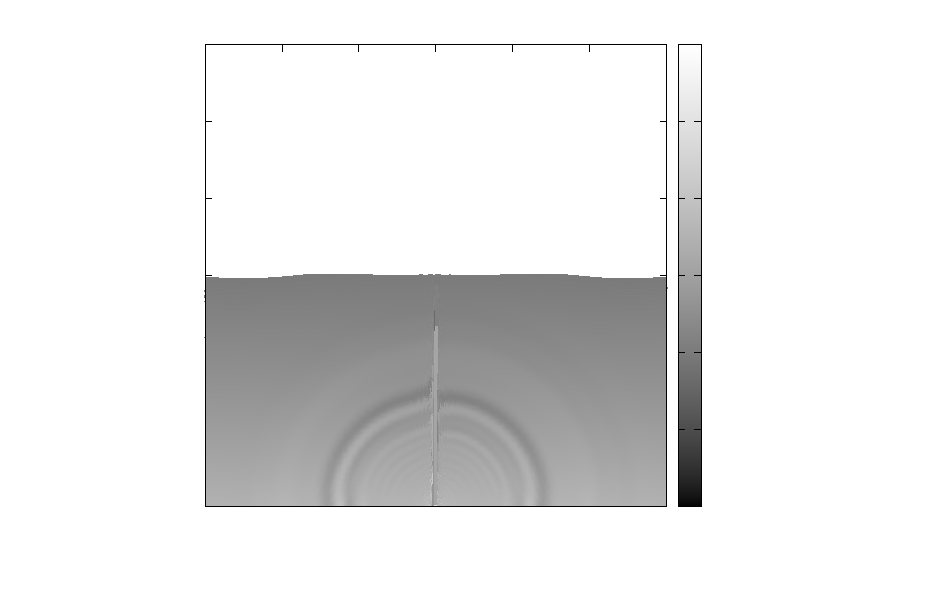
\includegraphics{./4Simulation/Shock1}}%
    \gplfronttext
  \end{picture}%
\endgroup

\caption{Initial shock-wave. $\tau  = 15.24$.}
\end{subfigure} \\
\begin{subfigure}{\textwidth}
% GNUPLOT: LaTeX picture with Postscript
\begingroup
  \makeatletter
  \providecommand\color[2][]{%
    \GenericError{(gnuplot) \space\space\space\@spaces}{%
      Package color not loaded in conjunction with
      terminal option `colourtext'%
    }{See the gnuplot documentation for explanation.%
    }{Either use 'blacktext' in gnuplot or load the package
      color.sty in LaTeX.}%
    \renewcommand\color[2][]{}%
  }%
  \providecommand\includegraphics[2][]{%
    \GenericError{(gnuplot) \space\space\space\@spaces}{%
      Package graphicx or graphics not loaded%
    }{See the gnuplot documentation for explanation.%
    }{The gnuplot epslatex terminal needs graphicx.sty or graphics.sty.}%
    \renewcommand\includegraphics[2][]{}%
  }%
  \providecommand\rotatebox[2]{#2}%
  \@ifundefined{ifGPcolor}{%
    \newif\ifGPcolor
    \GPcolorfalse
  }{}%
  \@ifundefined{ifGPblacktext}{%
    \newif\ifGPblacktext
    \GPblacktexttrue
  }{}%
  % define a \g@addto@macro without @ in the name:
  \let\gplgaddtomacro\g@addto@macro
  % define empty templates for all commands taking text:
  \gdef\gplbacktext{}%
  \gdef\gplfronttext{}%
  \makeatother
  \ifGPblacktext
    % no textcolor at all
    \def\colorrgb#1{}%
    \def\colorgray#1{}%
  \else
    % gray or color?
    \ifGPcolor
      \def\colorrgb#1{\color[rgb]{#1}}%
      \def\colorgray#1{\color[gray]{#1}}%
      \expandafter\def\csname LTw\endcsname{\color{white}}%
      \expandafter\def\csname LTb\endcsname{\color{black}}%
      \expandafter\def\csname LTa\endcsname{\color{black}}%
      \expandafter\def\csname LT0\endcsname{\color[rgb]{1,0,0}}%
      \expandafter\def\csname LT1\endcsname{\color[rgb]{0,1,0}}%
      \expandafter\def\csname LT2\endcsname{\color[rgb]{0,0,1}}%
      \expandafter\def\csname LT3\endcsname{\color[rgb]{1,0,1}}%
      \expandafter\def\csname LT4\endcsname{\color[rgb]{0,1,1}}%
      \expandafter\def\csname LT5\endcsname{\color[rgb]{1,1,0}}%
      \expandafter\def\csname LT6\endcsname{\color[rgb]{0,0,0}}%
      \expandafter\def\csname LT7\endcsname{\color[rgb]{1,0.3,0}}%
      \expandafter\def\csname LT8\endcsname{\color[rgb]{0.5,0.5,0.5}}%
    \else
      % gray
      \def\colorrgb#1{\color{black}}%
      \def\colorgray#1{\color[gray]{#1}}%
      \expandafter\def\csname LTw\endcsname{\color{white}}%
      \expandafter\def\csname LTb\endcsname{\color{black}}%
      \expandafter\def\csname LTa\endcsname{\color{black}}%
      \expandafter\def\csname LT0\endcsname{\color{black}}%
      \expandafter\def\csname LT1\endcsname{\color{black}}%
      \expandafter\def\csname LT2\endcsname{\color{black}}%
      \expandafter\def\csname LT3\endcsname{\color{black}}%
      \expandafter\def\csname LT4\endcsname{\color{black}}%
      \expandafter\def\csname LT5\endcsname{\color{black}}%
      \expandafter\def\csname LT6\endcsname{\color{black}}%
      \expandafter\def\csname LT7\endcsname{\color{black}}%
      \expandafter\def\csname LT8\endcsname{\color{black}}%
    \fi
  \fi
    \setlength{\unitlength}{0.0500bp}%
    \ifx\gptboxheight\undefined%
      \newlength{\gptboxheight}%
      \newlength{\gptboxwidth}%
      \newsavebox{\gptboxtext}%
    \fi%
    \setlength{\fboxrule}{0.5pt}%
    \setlength{\fboxsep}{1pt}%
\begin{picture}(8640.00,5400.00)%
    \gplgaddtomacro\gplbacktext{%
      \csname LTb\endcsname%
      \put(1677,704){\makebox(0,0)[r]{\strut{}$-15$}}%
      \put(1677,1443){\makebox(0,0)[r]{\strut{}$-10$}}%
      \put(1677,2181){\makebox(0,0)[r]{\strut{}$-5$}}%
      \put(1677,2920){\makebox(0,0)[r]{\strut{}$0$}}%
      \put(1677,3658){\makebox(0,0)[r]{\strut{}$5$}}%
      \put(1677,4397){\makebox(0,0)[r]{\strut{}$10$}}%
      \put(1677,5135){\makebox(0,0)[r]{\strut{}$15$}}%
      \put(1809,484){\makebox(0,0){\strut{}$-15$}}%
      \put(2548,484){\makebox(0,0){\strut{}$-10$}}%
      \put(3286,484){\makebox(0,0){\strut{}$-5$}}%
      \put(4025,484){\makebox(0,0){\strut{}$0$}}%
      \put(4764,484){\makebox(0,0){\strut{}$5$}}%
      \put(5502,484){\makebox(0,0){\strut{}$10$}}%
      \put(6241,484){\makebox(0,0){\strut{}$15$}}%
    }%
    \gplgaddtomacro\gplfronttext{%
      \csname LTb\endcsname%
      \put(1039,2919){\makebox(0,0){\strut{}$y$}}%
      \put(4025,154){\makebox(0,0){\strut{}$x$}}%
      \csname LTb\endcsname%
      \put(6705,704){\makebox(0,0)[l]{\strut{}$0.99$}}%
      \put(6705,1442){\makebox(0,0)[l]{\strut{}$0.995$}}%
      \put(6705,2181){\makebox(0,0)[l]{\strut{}$1$}}%
      \put(6705,2919){\makebox(0,0)[l]{\strut{}$1.005$}}%
      \put(6705,3657){\makebox(0,0)[l]{\strut{}$1.01$}}%
      \put(6705,4396){\makebox(0,0)[l]{\strut{}$1.015$}}%
      \put(6705,5134){\makebox(0,0)[l]{\strut{}$1.02$}}%
      \put(7431,2919){\makebox(0,0){\strut{} $\rho$}}%
    }%
    \gplbacktext
    \put(0,0){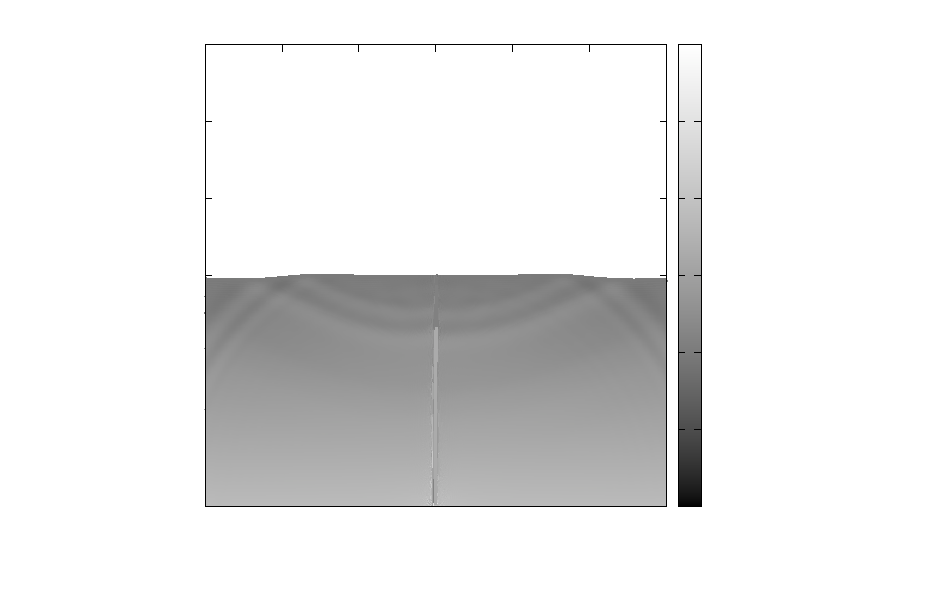
\includegraphics{Shock2}}%
    \gplfronttext
  \end{picture}%
\endgroup

\caption{Reflected shock-wave. $\tau = 15.56$.}
\end{subfigure}
\caption{Shock-wave created by primordial black hole leaving tank.}
\label{fig:shock}
\end{figure}

%\end{document}
